\documentclass[a4paper]{book}
\usepackage{makeidx}
\usepackage{natbib}
\usepackage{graphicx}
\usepackage{multicol}
\usepackage{float}
\usepackage{listings}
\usepackage{color}
\usepackage{ifthen}
\usepackage[table]{xcolor}
\usepackage{textcomp}
\usepackage{alltt}
\usepackage{ifpdf}
\ifpdf
\usepackage[pdftex,
            pagebackref=true,
            colorlinks=true,
            linkcolor=blue,
            unicode
           ]{hyperref}
\else
\usepackage[ps2pdf,
            pagebackref=true,
            colorlinks=true,
            linkcolor=blue,
            unicode
           ]{hyperref}
\usepackage{pspicture}
\fi
\usepackage[utf8]{inputenc}
\usepackage{polski}
\usepackage[T1]{fontenc}

\usepackage{mathptmx}
\usepackage[scaled=.90]{helvet}
\usepackage{courier}
\usepackage{sectsty}
\usepackage[titles]{tocloft}
\usepackage{doxygen}
\lstset{language=C++,inputencoding=utf8,basicstyle=\footnotesize,breaklines=true,breakatwhitespace=true,tabsize=8,numbers=left }
\makeindex
\setcounter{tocdepth}{3}
\renewcommand{\footrulewidth}{0.4pt}
\renewcommand{\familydefault}{\sfdefault}
\hfuzz=15pt
\setlength{\emergencystretch}{15pt}
\hbadness=750
\tolerance=750
\begin{document}
\hypersetup{pageanchor=false,citecolor=blue}
\begin{titlepage}
\vspace*{7cm}
\begin{center}
{\Large \-Mnozenie }\\
\vspace*{1cm}
{\large \-Wygenerowano przez Doxygen 1.7.6.1}\\
\vspace*{0.5cm}
{\small Sun Mar 2 2014 12:55:50}\\
\end{center}
\end{titlepage}
\clearemptydoublepage
\pagenumbering{roman}
\tableofcontents
\clearemptydoublepage
\pagenumbering{arabic}
\hypersetup{pageanchor=true,citecolor=blue}
\chapter{\-Indeks plików}
\section{\-Lista plików}
\-Tutaj znajduje się lista wszystkich plików z ich krótkimi opisami\-:\begin{DoxyCompactList}
\item\contentsline{section}{\hyperlink{funkcje_8cpp}{funkcje.\-cpp} }{\pageref{funkcje_8cpp}}{}
\item\contentsline{section}{\hyperlink{funkcje_8hh}{funkcje.\-hh} }{\pageref{funkcje_8hh}}{}
\item\contentsline{section}{\hyperlink{main_8cpp}{main.\-cpp} }{\pageref{main_8cpp}}{}
\end{DoxyCompactList}

\chapter{\-Dokumentacja plików}
\hypertarget{funkcje_8cpp}{\section{\-Dokumentacja pliku funkcje.\-cpp}
\label{funkcje_8cpp}\index{funkcje.\-cpp@{funkcje.\-cpp}}
}
{\ttfamily \#include \char`\"{}funkcje.\-hh\char`\"{}}\*
\-Wykres zależności załączania dla funkcje.\-cpp\-:\nopagebreak
\begin{figure}[H]
\begin{center}
\leavevmode
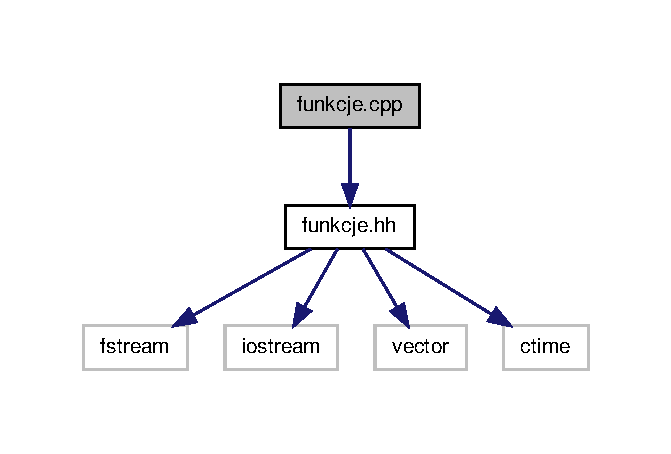
\includegraphics[width=322pt]{funkcje_8cpp__incl}
\end{center}
\end{figure}
\subsection*{\-Funkcje}
\begin{DoxyCompactItemize}
\item 
bool \hyperlink{funkcje_8cpp_ab80d311fc13e71453f3080482634447e}{otworz} (char $\ast$nazwa, fstream \&plik)
\item 
void \hyperlink{funkcje_8cpp_a7eac0a79b677c308c775f4f01aac9a6c}{kopiuj} (vector$<$ int $>$ \&wejsciowe, fstream \&plik, int rozmiar)
\begin{DoxyCompactList}\small\item\em kopiuje dane z pliku do wektora \end{DoxyCompactList}\item 
double \hyperlink{funkcje_8cpp_ad9ebe61e239dee170b242bda4db9ea63}{obliczenia} (const vector$<$ int $>$ \&wejsciowe, int $\ast$wyjsciowe, int powt)
\begin{DoxyCompactList}\small\item\em implementacja pomiatu czasu oraz algorytmu mnozenia \end{DoxyCompactList}\item 
void \hyperlink{funkcje_8cpp_aaa6c62fc60fb1173b904269379d69754}{zapisz} (int $\ast$tablica, fstream \&plik, int rozmiar)
\end{DoxyCompactItemize}


\subsection{\-Dokumentacja funkcji}
\hypertarget{funkcje_8cpp_a7eac0a79b677c308c775f4f01aac9a6c}{\index{funkcje.\-cpp@{funkcje.\-cpp}!kopiuj@{kopiuj}}
\index{kopiuj@{kopiuj}!funkcje.cpp@{funkcje.\-cpp}}
\subsubsection[{kopiuj}]{\setlength{\rightskip}{0pt plus 5cm}void {\bf kopiuj} (
\begin{DoxyParamCaption}
\item[{vector$<$ int $>$ \&}]{wejsciowe, }
\item[{fstream \&}]{plik, }
\item[{int}]{rozmiar}
\end{DoxyParamCaption}
)}}\label{funkcje_8cpp_a7eac0a79b677c308c775f4f01aac9a6c}
\-Funkcja pobiera wiersz danych z strumienia wejsciwego i zapisuje go w postaci zmiennej int do wektora 
\begin{DoxyParams}{\-Parametry}
{\em wejsciowe} & referencja wekstora przechowywujacego dane wejsciowe \\
\hline
{\em plik} & strumien wejscia zachaczony na pliku z danymi wejsciowymi \\
\hline
{\em rozmiar} & ilosc danych do przekopiowania \\
\hline
\end{DoxyParams}


\-Definicja w linii 27 pliku funkcje.\-cpp.



\-Oto graf wywoływań tej funkcji\-:\nopagebreak
\begin{figure}[H]
\begin{center}
\leavevmode
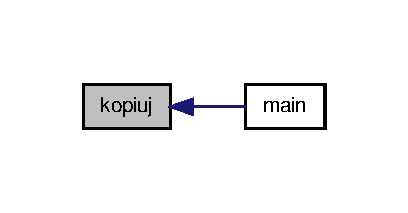
\includegraphics[width=196pt]{funkcje_8cpp_a7eac0a79b677c308c775f4f01aac9a6c_icgraph}
\end{center}
\end{figure}


\hypertarget{funkcje_8cpp_ad9ebe61e239dee170b242bda4db9ea63}{\index{funkcje.\-cpp@{funkcje.\-cpp}!obliczenia@{obliczenia}}
\index{obliczenia@{obliczenia}!funkcje.cpp@{funkcje.\-cpp}}
\subsubsection[{obliczenia}]{\setlength{\rightskip}{0pt plus 5cm}double {\bf obliczenia} (
\begin{DoxyParamCaption}
\item[{const vector$<$ int $>$ \&}]{wejsciowe, }
\item[{int $\ast$}]{wyjsciowe, }
\item[{int}]{powt}
\end{DoxyParamCaption}
)}}\label{funkcje_8cpp_ad9ebe61e239dee170b242bda4db9ea63}
w fuknkcji zostaje zmierzona ilość taktów procesora potrzebnych na wykonanie

zadanej ilości opercji mnożenia. \-Następnie ilość taktów zostaje podzielona przez

stała \-P\-E\-R\-\_\-\-T\-O\-\_\-\-S\-E\-C 
\begin{DoxyParams}{\-Parametry}
{\em wejsciowe} & dane ktore przetworzy algorytm \\
\hline
{\em wyjsciowe} & tablica wynikow mnozenia \\
\hline
{\em powt} & liczba powtorzen algorytmu \\
\hline
\end{DoxyParams}


\-Definicja w linii 47 pliku funkcje.\-cpp.



\-Oto graf wywoływań tej funkcji\-:
\nopagebreak
\begin{figure}[H]
\begin{center}
\leavevmode
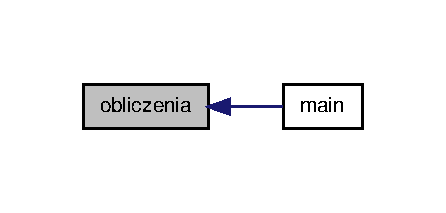
\includegraphics[width=214pt]{funkcje_8cpp_ad9ebe61e239dee170b242bda4db9ea63_icgraph}
\end{center}
\end{figure}


\hypertarget{funkcje_8cpp_ab80d311fc13e71453f3080482634447e}{\index{funkcje.\-cpp@{funkcje.\-cpp}!otworz@{otworz}}
\index{otworz@{otworz}!funkcje.cpp@{funkcje.\-cpp}}
\subsubsection[{otworz}]{\setlength{\rightskip}{0pt plus 5cm}bool {\bf otworz} (
\begin{DoxyParamCaption}
\item[{char $\ast$}]{nazwa, }
\item[{fstream \&}]{plik}
\end{DoxyParamCaption}
)}}\label{funkcje_8cpp_ab80d311fc13e71453f3080482634447e}


\-Definicja w linii 13 pliku funkcje.\-cpp.



\-Oto graf wywoływań tej funkcji\-:\nopagebreak
\begin{figure}[H]
\begin{center}
\leavevmode
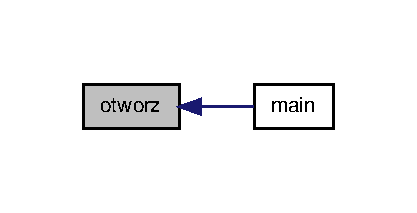
\includegraphics[width=200pt]{funkcje_8cpp_ab80d311fc13e71453f3080482634447e_icgraph}
\end{center}
\end{figure}


\hypertarget{funkcje_8cpp_aaa6c62fc60fb1173b904269379d69754}{\index{funkcje.\-cpp@{funkcje.\-cpp}!zapisz@{zapisz}}
\index{zapisz@{zapisz}!funkcje.cpp@{funkcje.\-cpp}}
\subsubsection[{zapisz}]{\setlength{\rightskip}{0pt plus 5cm}void {\bf zapisz} (
\begin{DoxyParamCaption}
\item[{int $\ast$}]{tablica, }
\item[{fstream \&}]{plik, }
\item[{int}]{rozmiar}
\end{DoxyParamCaption}
)}}\label{funkcje_8cpp_aaa6c62fc60fb1173b904269379d69754}


\-Definicja w linii 75 pliku funkcje.\-cpp.



\-Oto graf wywoływań tej funkcji\-:\nopagebreak
\begin{figure}[H]
\begin{center}
\leavevmode
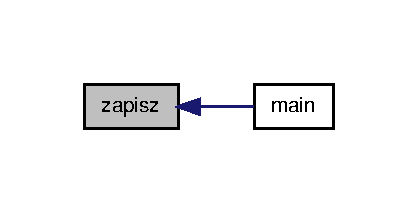
\includegraphics[width=200pt]{funkcje_8cpp_aaa6c62fc60fb1173b904269379d69754_icgraph}
\end{center}
\end{figure}



\hypertarget{funkcje_8hh}{\section{\-Dokumentacja pliku funkcje.\-hh}
\label{funkcje_8hh}\index{funkcje.\-hh@{funkcje.\-hh}}
}
{\ttfamily \#include $<$fstream$>$}\*
{\ttfamily \#include $<$iostream$>$}\*
{\ttfamily \#include $<$vector$>$}\*
{\ttfamily \#include $<$ctime$>$}\*
\-Wykres zależności załączania dla funkcje.\-hh\-:\nopagebreak
\begin{figure}[H]
\begin{center}
\leavevmode
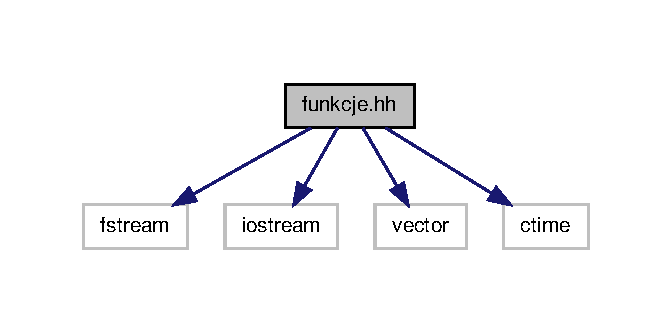
\includegraphics[width=322pt]{funkcje_8hh__incl}
\end{center}
\end{figure}
\-Ten wykres pokazuje, które pliki bezpośrednio lub pośrednio załączają ten plik\-:\nopagebreak
\begin{figure}[H]
\begin{center}
\leavevmode
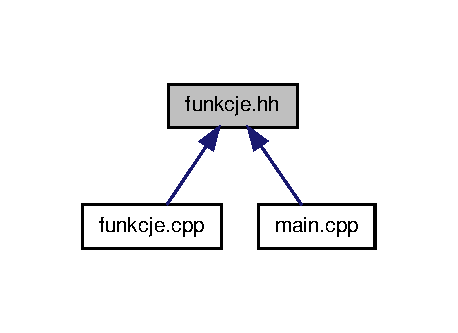
\includegraphics[width=220pt]{funkcje_8hh__dep__incl}
\end{center}
\end{figure}
\subsection*{\-Definicje}
\begin{DoxyCompactItemize}
\item 
\#define \hyperlink{funkcje_8hh_a3d9fc3c745d0880902fe3ea3d5d5f71e}{\-C\-L\-O\-C\-K\-S\-\_\-\-P\-E\-R\-\_\-\-S\-E\-C}~1000000
\end{DoxyCompactItemize}
\subsection*{\-Funkcje}
\begin{DoxyCompactItemize}
\item 
void \hyperlink{funkcje_8hh_aaa6c62fc60fb1173b904269379d69754}{zapisz} (int $\ast$tablica, fstream \&plik, int rozmiar)
\item 
double \hyperlink{funkcje_8hh_ad9ebe61e239dee170b242bda4db9ea63}{obliczenia} (const vector$<$ int $>$ \&wejsciowe, int $\ast$wyjsciowe, int powt)
\begin{DoxyCompactList}\small\item\em implementacja pomiatu czasu oraz algorytmu mnozenia \end{DoxyCompactList}\item 
bool \hyperlink{funkcje_8hh_ab80d311fc13e71453f3080482634447e}{otworz} (char $\ast$nazwa, fstream \&plik)
\item 
void \hyperlink{funkcje_8hh_a7eac0a79b677c308c775f4f01aac9a6c}{kopiuj} (vector$<$ int $>$ \&wejsciowe, fstream \&plik, int rozmiar)
\begin{DoxyCompactList}\small\item\em kopiuje dane z pliku do wektora \end{DoxyCompactList}\end{DoxyCompactItemize}


\subsection{\-Dokumentacja definicji}
\hypertarget{funkcje_8hh_a3d9fc3c745d0880902fe3ea3d5d5f71e}{\index{funkcje.\-hh@{funkcje.\-hh}!\-C\-L\-O\-C\-K\-S\-\_\-\-P\-E\-R\-\_\-\-S\-E\-C@{\-C\-L\-O\-C\-K\-S\-\_\-\-P\-E\-R\-\_\-\-S\-E\-C}}
\index{\-C\-L\-O\-C\-K\-S\-\_\-\-P\-E\-R\-\_\-\-S\-E\-C@{\-C\-L\-O\-C\-K\-S\-\_\-\-P\-E\-R\-\_\-\-S\-E\-C}!funkcje.hh@{funkcje.\-hh}}
\subsubsection[{\-C\-L\-O\-C\-K\-S\-\_\-\-P\-E\-R\-\_\-\-S\-E\-C}]{\setlength{\rightskip}{0pt plus 5cm}\#define {\bf \-C\-L\-O\-C\-K\-S\-\_\-\-P\-E\-R\-\_\-\-S\-E\-C}~1000000}}\label{funkcje_8hh_a3d9fc3c745d0880902fe3ea3d5d5f71e}


\-Definicja w linii 14 pliku funkcje.\-hh.



\subsection{\-Dokumentacja funkcji}
\hypertarget{funkcje_8hh_a7eac0a79b677c308c775f4f01aac9a6c}{\index{funkcje.\-hh@{funkcje.\-hh}!kopiuj@{kopiuj}}
\index{kopiuj@{kopiuj}!funkcje.hh@{funkcje.\-hh}}
\subsubsection[{kopiuj}]{\setlength{\rightskip}{0pt plus 5cm}void {\bf kopiuj} (
\begin{DoxyParamCaption}
\item[{vector$<$ int $>$ \&}]{wejsciowe, }
\item[{fstream \&}]{plik, }
\item[{int}]{rozmiar}
\end{DoxyParamCaption}
)}}\label{funkcje_8hh_a7eac0a79b677c308c775f4f01aac9a6c}
\-Funkcja pobiera wiersz danych z strumienia wejsciwego i zapisuje go w postaci zmiennej int do wektora 
\begin{DoxyParams}{\-Parametry}
{\em wejsciowe} & referencja wekstora przechowywujacego dane wejsciowe \\
\hline
{\em plik} & strumien wejscia zachaczony na pliku z danymi wejsciowymi \\
\hline
{\em rozmiar} & ilosc danych do przekopiowania \\
\hline
\end{DoxyParams}


\-Definicja w linii 27 pliku funkcje.\-cpp.



\-Oto graf wywoływań tej funkcji\-:\nopagebreak
\begin{figure}[H]
\begin{center}
\leavevmode
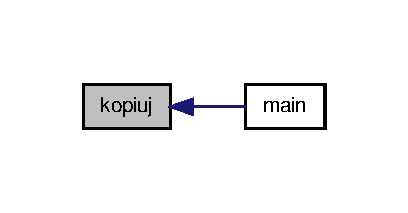
\includegraphics[width=196pt]{funkcje_8hh_a7eac0a79b677c308c775f4f01aac9a6c_icgraph}
\end{center}
\end{figure}


\hypertarget{funkcje_8hh_ad9ebe61e239dee170b242bda4db9ea63}{\index{funkcje.\-hh@{funkcje.\-hh}!obliczenia@{obliczenia}}
\index{obliczenia@{obliczenia}!funkcje.hh@{funkcje.\-hh}}
\subsubsection[{obliczenia}]{\setlength{\rightskip}{0pt plus 5cm}double {\bf obliczenia} (
\begin{DoxyParamCaption}
\item[{const vector$<$ int $>$ \&}]{wejsciowe, }
\item[{int $\ast$}]{wyjsciowe, }
\item[{int}]{powt}
\end{DoxyParamCaption}
)}}\label{funkcje_8hh_ad9ebe61e239dee170b242bda4db9ea63}
w fuknkcji zostaje zmierzona ilość taktów procesora potrzebnych na wykonanie

zadanej ilości opercji mnożenia. \-Następnie ilość taktów zostaje podzielona przez

stała \-P\-E\-R\-\_\-\-T\-O\-\_\-\-S\-E\-C 
\begin{DoxyParams}{\-Parametry}
{\em wejsciowe} & dane ktore przetworzy algorytm \\
\hline
{\em wyjsciowe} & tablica wynikow mnozenia \\
\hline
{\em powt} & liczba powtorzen algorytmu \\
\hline
\end{DoxyParams}


\-Definicja w linii 47 pliku funkcje.\-cpp.



\-Oto graf wywoływań tej funkcji\-:
\nopagebreak
\begin{figure}[H]
\begin{center}
\leavevmode
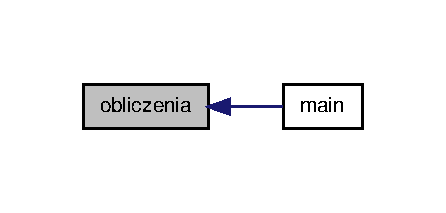
\includegraphics[width=214pt]{funkcje_8hh_ad9ebe61e239dee170b242bda4db9ea63_icgraph}
\end{center}
\end{figure}


\hypertarget{funkcje_8hh_ab80d311fc13e71453f3080482634447e}{\index{funkcje.\-hh@{funkcje.\-hh}!otworz@{otworz}}
\index{otworz@{otworz}!funkcje.hh@{funkcje.\-hh}}
\subsubsection[{otworz}]{\setlength{\rightskip}{0pt plus 5cm}bool {\bf otworz} (
\begin{DoxyParamCaption}
\item[{char $\ast$}]{nazwa, }
\item[{fstream \&}]{plik}
\end{DoxyParamCaption}
)}}\label{funkcje_8hh_ab80d311fc13e71453f3080482634447e}


\-Definicja w linii 13 pliku funkcje.\-cpp.



\-Oto graf wywoływań tej funkcji\-:\nopagebreak
\begin{figure}[H]
\begin{center}
\leavevmode
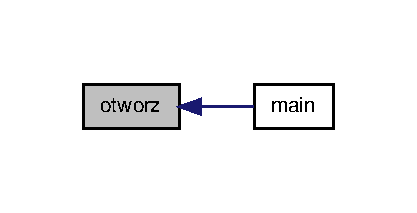
\includegraphics[width=200pt]{funkcje_8hh_ab80d311fc13e71453f3080482634447e_icgraph}
\end{center}
\end{figure}


\hypertarget{funkcje_8hh_aaa6c62fc60fb1173b904269379d69754}{\index{funkcje.\-hh@{funkcje.\-hh}!zapisz@{zapisz}}
\index{zapisz@{zapisz}!funkcje.hh@{funkcje.\-hh}}
\subsubsection[{zapisz}]{\setlength{\rightskip}{0pt plus 5cm}void {\bf zapisz} (
\begin{DoxyParamCaption}
\item[{int $\ast$}]{tablica, }
\item[{fstream \&}]{plik, }
\item[{int}]{rozmiar}
\end{DoxyParamCaption}
)}}\label{funkcje_8hh_aaa6c62fc60fb1173b904269379d69754}


\-Definicja w linii 75 pliku funkcje.\-cpp.



\-Oto graf wywoływań tej funkcji\-:\nopagebreak
\begin{figure}[H]
\begin{center}
\leavevmode
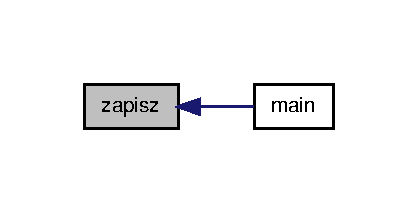
\includegraphics[width=200pt]{funkcje_8hh_aaa6c62fc60fb1173b904269379d69754_icgraph}
\end{center}
\end{figure}



\hypertarget{main_8cpp}{\section{\-Dokumentacja pliku main.\-cpp}
\label{main_8cpp}\index{main.\-cpp@{main.\-cpp}}
}
{\ttfamily \#include \char`\"{}iostream\char`\"{}}\*
{\ttfamily \#include \char`\"{}funkcje.\-hh\char`\"{}}\*
{\ttfamily \#include $<$fstream$>$}\*
{\ttfamily \#include $<$vector$>$}\*
\-Wykres zależności załączania dla main.\-cpp\-:\nopagebreak
\begin{figure}[H]
\begin{center}
\leavevmode
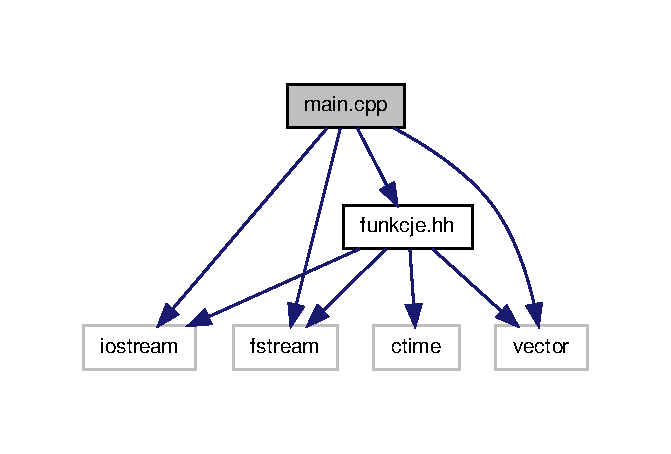
\includegraphics[width=322pt]{main_8cpp__incl}
\end{center}
\end{figure}
\subsection*{\-Funkcje}
\begin{DoxyCompactItemize}
\item 
int \hyperlink{main_8cpp_ae66f6b31b5ad750f1fe042a706a4e3d4}{main} ()
\end{DoxyCompactItemize}
\subsection*{\-Zmienne}
\begin{DoxyCompactItemize}
\item 
fstream \hyperlink{main_8cpp_a51b2d7dd921655a19be32f545416083f}{dane}
\item 
fstream \hyperlink{main_8cpp_a67ff2f1724c27ce37872c5d75172f4ff}{wynik}
\item 
ofstream \hyperlink{main_8cpp_a70c6fb164e3ab54a6815de7a9e562b7b}{czas}
\end{DoxyCompactItemize}


\subsection{\-Dokumentacja funkcji}
\hypertarget{main_8cpp_ae66f6b31b5ad750f1fe042a706a4e3d4}{\index{main.\-cpp@{main.\-cpp}!main@{main}}
\index{main@{main}!main.cpp@{main.\-cpp}}
\subsubsection[{main}]{\setlength{\rightskip}{0pt plus 5cm}int {\bf main} (
\begin{DoxyParamCaption}
{}
\end{DoxyParamCaption}
)}}\label{main_8cpp_ae66f6b31b5ad750f1fe042a706a4e3d4}


\-Definicja w linii 21 pliku main.\-cpp.



\-Oto graf wywołań dla tej funkcji\-:
\nopagebreak
\begin{figure}[H]
\begin{center}
\leavevmode
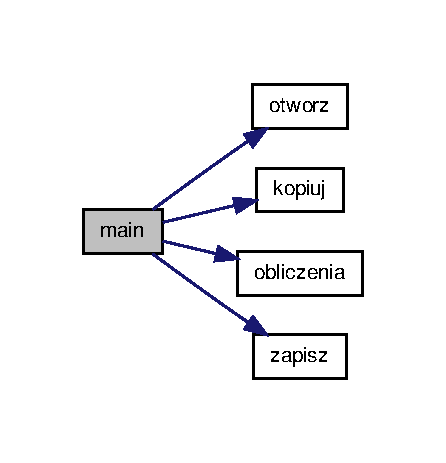
\includegraphics[width=214pt]{main_8cpp_ae66f6b31b5ad750f1fe042a706a4e3d4_cgraph}
\end{center}
\end{figure}




\subsection{\-Dokumentacja zmiennych}
\hypertarget{main_8cpp_a70c6fb164e3ab54a6815de7a9e562b7b}{\index{main.\-cpp@{main.\-cpp}!czas@{czas}}
\index{czas@{czas}!main.cpp@{main.\-cpp}}
\subsubsection[{czas}]{\setlength{\rightskip}{0pt plus 5cm}ofstream {\bf czas}}}\label{main_8cpp_a70c6fb164e3ab54a6815de7a9e562b7b}


\-Definicja w linii 19 pliku main.\-cpp.

\hypertarget{main_8cpp_a51b2d7dd921655a19be32f545416083f}{\index{main.\-cpp@{main.\-cpp}!dane@{dane}}
\index{dane@{dane}!main.cpp@{main.\-cpp}}
\subsubsection[{dane}]{\setlength{\rightskip}{0pt plus 5cm}fstream {\bf dane}}}\label{main_8cpp_a51b2d7dd921655a19be32f545416083f}


\-Definicja w linii 17 pliku main.\-cpp.

\hypertarget{main_8cpp_a67ff2f1724c27ce37872c5d75172f4ff}{\index{main.\-cpp@{main.\-cpp}!wynik@{wynik}}
\index{wynik@{wynik}!main.cpp@{main.\-cpp}}
\subsubsection[{wynik}]{\setlength{\rightskip}{0pt plus 5cm}fstream {\bf wynik}}}\label{main_8cpp_a67ff2f1724c27ce37872c5d75172f4ff}


\-Definicja w linii 18 pliku main.\-cpp.


\printindex
\end{document}
